\documentclass[%
reprint,
superscriptaddress,
%groupedaddress,
%unsortedaddress,
%runinaddress,
%frontmatterverbose,
%preprint,
showpacs,preprintnumbers,
%nofootinbib,
%nobibnotes,
%bibnotes,
 amsmath,amssymb,
 aps,
%pra,
%prb,
prd,
%prl,
%rmp,
%prstab,
%prstper,
%floatfix,
]{revtex4-1}

\usepackage{float}
\usepackage{graphicx}% Include figure files
\usepackage{dcolumn}% Align table columns on decimal point
\usepackage{bm}% bold math
\usepackage{bbold}
\usepackage{braket}
\usepackage{amssymb,amsmath}
\usepackage{hyperref}% add hypertext capabilities
%\usepackage[mathlines]{lineno}% Enable numbering of text and display math
%\linenumbers\relax % Commence numbering lines

%\usepackage[showframe,%Uncomment any one of the following lines to test
%%scale=0.7, marginratio={1:1, 2:3}, ignoreall,% default settings
%%text={7in,10in},centering,
%%margin=1.5in,
%%total={6.5in,8.75in}, top=1.2in, left=0.9in, includefoot,
%%height=10in,a5paper,hmargin={3cm,0.8in},
%]{geometry}



\usepackage{color}
\usepackage[dvipsnames, svgnames, x11names]{xcolor}
\usepackage{amsfonts}
\usepackage{subfigure}
\usepackage{array}


\newcommand{\Tr}{\ensuremath{\operatorname{Tr}}}
\newcommand{\tr}{\ensuremath{\operatorname{tr}}}
\newcommand{\Omegaqq}{\ensuremath{\Omega_{\bar{q}q}}}
\newcommand{\vev}[1]{\ensuremath{\left\langle #1 \right\rangle}}
\newcommand{\einh}[1]{\ensuremath{\,\text{#1}}}
\newcolumntype{L}{>{\centering\arraybackslash}m{3cm}}



\newcommand{\overbar}[1]{\mkern 1.5mu\overline{\mkern-1.5mu#1\mkern-1.5mu}\mkern 1.5mu}

\definecolor{bjcol}{rgb}{1,.44,0.13}

% color def's

\definecolor{blue}{rgb}{0,0,1}
\newcommand{\colb}[1]{{\color{blue} #1}}
\definecolor{green}{rgb}{0,1,0}
\newcommand{\colg}[1]{{\color{green} #1}}
\definecolor{red}{rgb}{1,0,0}
\newcommand{\colr}[1]{{\color{red} #1}}
\newcommand{\colJ}[1]{{\color{cyan} #1}}
\definecolor{gray}{rgb}{.5,.5,.5}
\newcommand{\drop}[1]{{\sout{ {\color{gray} #1}}}}
\definecolor{darkgreen}{rgb}{.0,.5,.0}
\newcommand{\colL}[1]{{\color{darkgreen} #1}}


\def\Fig#1{Fig.~\ref{#1}} \def\Tab#1{Tab.~\ref{#1}}
\def\Figs#1{Figs.~\ref{#1}} \def\Tab#1{Tab.~\ref{#1}}
\def\Eqs#1{Eqs.~(\ref{#1})}
\def\Eq#1{Eq.~(\ref{#1})}
\def\eq#1{(\ref{#1})}
\def\eqref#1{(\ref{#1})}
\def\fig#1{Fig.~\ref{#1}}
\def\tab#1{Tab.~\ref{#1}}
\def\eqs#1{(\ref{#1})}
\def\Eqs#1{(\ref{#1})}
\def\sec#1{Sec.~\ref{#1}}
\def\app#1{Appendix~\ref{#1}}
\newcommand{\Phibar}{\ensuremath{\bar{\Phi}}}
\newcommand{\LPQM}{\ensuremath{\mathcal{L}_{\textrm{PQM}}}\xspace}

\def\dbar{{\mathchar'26\mkern-12mu d}}
\def\lA0{{\langle A_0 \rangle}}
\def\bA0{{\bar{A}_0}}
\def\lLA{{\langle L[A_0] \rangle}}
\def\lL{{\langle L \rangle}}
\def\lLc{{\langle L^\dagger \rangle}}
\def\lLAc{{\langle L^\dagger[A_0] \rangle}}


\def\dr{{D\!\llap{/}}\,}
\def\Dr{{D\!\llap{/}}\,}
\def\ipv{\vec{p}\llap{/}}
\def\pslash{p\llap{/}}

\def\0#1#2{\frac{#1}{#2}}

\newcommand{\bsig}{\ensuremath{\bar{\sigma}}}
\newcommand{\lsm}{L\ensuremath{\sigma}M\xspace}
\newcommand{\pT}{\ensuremath{T_0}}
\newcommand{\Tl}{\ensuremath{T_\chi}}
\newcommand{\Ts}{\ensuremath{T_\chi^s}}
\newcommand{\Tchi}{\ensuremath{T_\chi}}
\newcommand{\Td}{\ensuremath{T_d}}
\newcommand{\Tc}{\ensuremath{T_c}}
\newcommand{\muc}{\ensuremath{\mu_c}}
\newcommand{\coloronl}{(color online)\xspace}

\newcommand{\mrm}[1]{\mathrm{#1}}
\def\qbar{\bar{q}}
\newcommand{\sx}{\sigma_{x}}
\newcommand{\sy}{\sigma_{y}}

%%%%%%%%%%%%%% for corrections %%%%%%%%%%%
\newcommand{\colwj}[1]{\textcolor{Purple}{#1}}
\newcommand{\colxf}[1]{\textcolor{cyan}{#1}}
\newcommand{\coljan}[1]{\textcolor{red}{#1}}
\newcommand{\colfabian}[1]{\textcolor{magenta}{#1}}
\newcommand{\colrui}[1]{\textcolor{green}{#1}}
\newcommand{\colnu}[1]{\textcolor{blue}{#1}}
\newcommand{\colshi}[1]{\textcolor{Plum}{#1}}

%
%%%%%%%%%%%%%%%%%%%%%%%%%%%%%%%%%%%%%%%%%%%%%%%%%%%%%%%%%%%%%%%%%%%%%%%%%%%%%

\graphicspath{{./figures/}{./}}

\begin{document}

\preprint{}

\title{Hyper-order baryon number fluctuations at finite temperature and density}


\author{Wei-jie Fu}
\affiliation{School of Physics, Dalian University of Technology, Dalian, 116024,
  P.R. China}

\author{Xiaofeng Luo}
\affiliation{Key Laboratory of Quark \& Lepton Physics (MOE) and Institute of Particle Physics,
Central China Normal University, Wuhan 430079, China}

\author{Jan M. Pawlowski}
\affiliation{Institut f\"ur Theoretische Physik, Universit\"at Heidelberg, Philosophenweg 16, 69120 Heidelberg, Germany}
\affiliation{ExtreMe Matter Institute EMMI, GSI, Planckstra{\ss}e 1, D-64291 Darmstadt, Germany}

\author{Fabian Rennecke}
\affiliation{Physics Department, Brookhaven National Laboratory, Upton, NY 11973, USA}

\author{Rui Wen}
\affiliation{School of Physics, Dalian University of Technology, Dalian, 116024,
  P.R. China}

\author{Nu Xu}
\affiliation{Key Laboratory of Quark \& Lepton Physics (MOE) and Institute of Particle Physics,
Central China Normal University, Wuhan 430079, China}
\affiliation{Lawrence Berkeley National Laboratory, Berkeley, CA 94720, USA}
\affiliation{Institute of Modern Physics of CAS, Lanzhou 730000, China}

\author{Shi Yin}
\affiliation{School of Physics, Dalian University of Technology, Dalian, 116024,
  P.R. China}


%\date{\today}% It is always \today, today,
             %  but any date may be explicitly specified

\begin{abstract}
We study the generalized susceptibilities from kurtosis which is known as the $\chi^B_4/\chi^B_2$ to the $\chi^B_8/\chi^B_2$. The results are obtained under the finite temperature and baryon density. We give the comparison of our results with the lattice QCD results under the vanishing $\mu_B$. We get the numerical results under the Polyakov-quark-meson (PQM) model with the functional renormalisation group (FRG) approch.


\end{abstract}
%\pacs{Valid PACS appear here}% PACS, the Physics and Astronomy
\pacs{11.30.Rd, %Chiral symmetries
         11.10.Wx, %Finite-temperature field theory
         05.10.Cc, %Renormalization group methods
         12.38.Mh  %Quark-gluon plasma
     }                             % Classification Scheme.
%\keywords{Suggested keywords}%Use showkeys class option if keyword
                              %display desired
\maketitle
%\tableofcontents

%%%%%%%%%%%%%%%%%%%%%%%%%%%%%%%%%%%%%%%%%%%%%%%%%%%%%%%%%%%
%%%%%%%%%%%%%%%%%%%%%%%%%%%%%%%%%%%%%%%%%%%%%%%%%%%%%%%%%%%

\section{Introduction}
\label{sec:int}









%%%%%%%%%%%%%%%%%%%%%%%%%%%%%%%%%%%%%%%%%%%%%%%%%%%%%%%%%%%%%
%%%%%%%%%%%%%%%%%%%%%%%%%%%%%%%%%%%%%%%%%%%%%%%%%%%%%%%%%%%%%

\section{QCD and low energy effective theories within the fRG approach}
\label{sec:FRG}

%
 %%%%%%%%%%%%%%%%%%%%%%%%%%%%
\begin{figure}[t]
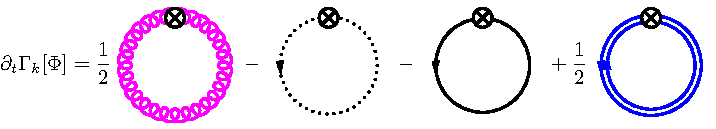
\includegraphics[width=0.45\textwidth]{QCD_equation}
\caption{Diagrammatic representation of the QCD flow equation within the fRG approach. Lines of different types on the r.h.s. of the equation stand for the full propagators of gluon, ghost, quark, and meson, respectively. Note that the mesonic degree of freedom is denoted by double lines with opposite arrows. The crossed circles represent the regulators in the flow equation.}\label{fig:QCD_equation}
\end{figure}
%%%%%%%%%%%%%%%%%%%%%%%%%%%%%
%

An generic Euclidian quantum field theory is completely described by its effective action $\Gamma[\Phi]$, where $\Phi$ is used to denote an aggregate of all fields in the theory. In the fRG approach, this full quantum effective action is resolved by  
interpolating it as a function of a renormalization group (RG) scale $k$, i.e.,  $\Gamma_k[\Phi]$, successively, starting from the respective classical action $S[\Phi]$ at a very high ultraviolet (UV) scale, say $\Lambda$, towards the infrared (IR) limit $k\rightarrow 0$ with $\Gamma[\Phi]=\Gamma_{k=0}[\Phi]$. For more details about the formalism of fRG, see, e.g., \cite{Wetterich:1992yh} as well as \cite{Ellwanger:1993mw,Morris:1993qb}. 

To be specific, the flow equation for QCD, which describes the evolution of its effective action with the RG scale $k$, is shown in \Fig{fig:QCD_equation} diagrammatically. As one could see, the QCD flow receives contributions not only from the  gluon, ghost and the quark, i.e., the fundamental partonic degrees of freedom in QCD, but also from hadrons, such as mesons, which are composite or emergent degrees of freedom, and are generated dynamically through strong interactions when the RG scale is reduced down to the nonperturbative regime of the low energy QCD. Recent first-principle QCD calculations within fRG indicate that this transition, from the partonic to composite degrees of freedom, takes place in a narrow regime located at $k\sim$1 GeV \cite{Mitter:2014wpa,Braun:2014ata,Cyrol:2017ewj,Fu:2019hdw}. The flow of the QCD effective action corresponding to the diagrams in \Fig{fig:QCD_equation} can be written as follows,
%
\begin{align}
\partial_t\Gamma_k[\Phi]=&\frac{1}{2}\mathrm{Tr}\Big(G_{AA,k}\partial_t R_{A,k}\Big)-\mathrm{Tr}\Big(G_{c\bar c,k}\partial_t R_{c,k}\Big)\nonumber\\[2ex]
  &-\mathrm{Tr}\Big(G_{q\bar q,k}\partial_t R_{q,k}\Big)+\frac{1}{2}\mathrm{Tr}\Big(G_{\phi\phi,k}\partial_t R_{\phi,k}\Big)\,,\label{eq:QCDflow}
\end{align}
%
with $\Phi=(A, c, \bar c, q,\bar q,\phi)$, where $G$'s and $R$'s are the propagators and regulators of different fields, respectively. Note that the scale dependence of these quantities is explicitly indicated with a suffix $k$. The RG time in \Eq{eq:QCDflow} is defined by $t=\ln(k/\Lambda)$, with the initial UV scale $\Lambda$. We are not going to discuss details of the QCD flow in \Eq{eq:QCDflow} here, and interested readers are strongly suggested to refer to, e.g.,  \cite{Braun:2007bx,Braun:2008pi,Braun:2009gm,Mitter:2014wpa,Braun:2014ata,Cyrol:2016tym,Cyrol:2017ewj,Cyrol:2017qkl,Fu:2019hdw,Braun:2020ada} for recent progress in understanding of QCD or Yang-Mills theory in the vacuum and at finite temperature and density within the fRG approach, and also \cite{Berges:2000ew,Pawlowski:2005xe,Schaefer:2006sr,Gies:2006wv,Rosten:2010vm,Braun:2011pp,Pawlowski:2014aha} for QCD related review articles of fRG.

As mentioned above, the transition of the degrees of freedom, from the partonic ones in the perturbative regime of high energy to the hadronic ones in the nonperturbative region of low energy, is realized through the dynamical hadronization in the fRG approach. With the help of the technique of dynamical hadronization, composite operators of resonated channels, e.g., the $\sigma$-$\pi$ channel, i.e., the scalar-pseudoscalar one in the low energy QCD, which are most relevant to the dynamics of the system, are bosonized or Hubbard-Stratonovich transformed successively with the evolution of RG scale. For more details, see, e.g., \cite{Gies:2001nw,Gies:2002hq,Pawlowski:2005xe,Floerchinger:2009uf,Fu:2019hdw}. 

In a recent first-principle fRG calculation to QCD, it has been shown clearly that a sequential decoupling of the gluon, quark, and mesonic degrees of freedom from the system with decreasing RG scale, results in a natural emergence of the low energy effective theory (LEFT) when the scale $k\lesssim 1$ GeV \cite{Fu:2019hdw}. The fRG formalism is ideally suited to the description of a phenomenon of emergence, which usually involves energy scale of different hierarchies, characteristic to different degrees of freedom. When the scale $k$ is high and the system is located in the perturbative region, the only relevant degrees of freedom in QCD are the gluon and quark, and the hadronic or mesonic ones are irrelevant due to their large masses. When $k$ decreases below $\sim 1$ GeV, the gluon develops a significant mass gap in the low momentum region, and thus decouples from the system. The dynamics is taken over by the emergent composite degrees of freedom, e.g. mesons, in particular the $\pi$ meson, which is in essence the Goldstone boson related to the spontaneously breaking chiral symmetry in the low energy QCD, and is the lightest hadron of mass $\sim 140$ MeV in the vacuum. 

The direct consequence of the natural emergence of LEFT is that,  if the flow equation of QCD in \Eq{eq:QCDflow} is evolved at a starting scale, in which the glue sector has already significantly been suppressed by the gluon mass gap, say $\Lambda \sim 1$ GeV, it is safe and legitimate to disregard quantum fluctuations of the glue sector, i.e., the first two diagrams in \Fig{fig:QCD_equation}. Hence we are left with a scale dependent effective action, only composed of the matter sector fields, namely, the quark and meson, which reads
%
\begin{align}
\Gamma_k[\Phi]=&\int_x \bigg\{Z_{q,k}\bar{q} \Big [\gamma_\mu \partial_\mu -\gamma_0(\hat\mu+igA_0) \Big ]q+\frac{1}{2}Z_{\phi,k}(\partial_\mu \phi)^2 \nonumber\\[2ex]
&+h_k\bar{q}\big(T^0\sigma+i\gamma_5\vec{T}\cdot \vec{\pi}\big)q+V_k(\rho,A_0)-c\sigma \bigg\}\,,\label{eq:action}
\end{align}
%
with a reduction of the involved species of fields $\Phi=(q,\bar q,\phi)$, and the shorthand notation for the space-time integral $\int_{x}=\int_0^{1/T}d x_0 \int d^3 x$. Note that in this work we only consider the case of $N_f=2$ flavor quark, i.e., the quark field $q=(u\,,d)^{T}$ in the action \Eq{eq:action}. The meson field $\phi=\left(\sigma,\vec{\pi}\right)$, being in the adjoint representation of group $\mathrm{U_V}(N_f)\times\mathrm{U_A}(N_f)$ in the flavor space, is coupled with the quark field through the Yukawa coupling. Here $T^0$ and $T^{i}$'s ($i=1\,,2\,,\cdots\,,N_f^2-1$) are the generators of $\mathrm{U}(N_f)$ group, denoted collectively as $T^a$'s, with the normalization $\Tr(T^{a}T^{b})=\frac{1}{2}\delta^{ab}$, which yields $T^{0}=\frac{1}{\sqrt{2N_{f}}}\mathbb{1}_{N_{f}\times N_{f}}$. $Z_{q,k}$ and $Z_{\phi,k}$ are the wave function renormalization for the quark and meson fields, respectively. Note that the wave function renormalizations, as well as the Yukawa coupling $h_k$ and the effective potential $V_k$ to be discussed in the following, are dependent on the RG scale $k$. 

Quantum fluctuations of the glue sector are suppressed in the low energy region due to the large gluon mass gap as discussed above, and consequently it is reasonable to neglect their corresponding contributions in the flow equation of QCD in \Fig{fig:QCD_equation} or \Eq{eq:QCDflow}. The gluonic background field is, however, of significant importance for the QCD thermodynamics. In \Eq{eq:action} the temporal component of the gluonic background field $A_0$ is encoded, which is responsible for the quark confinement in the statistical sense of thermodynamics, see, e.g., \cite{Fukushima:2003fw,Ratti:2005jh,Schaefer:2007pw,Fu:2007xc} for more details. Therefore, the effective potential in \Eq{eq:action} reads
%
\begin{align}
V_k(\rho,A_0)=&V_{\mathrm{glue},k}(A_0)+V_{\mathrm{mat},k}(\rho,A_0)\,,\label{eq:Vtotal}
\end{align}
%
where the first term on the right-hand side is due to the temporal gluonic background field $A_0$, which can also be formulated in terms of the Polyakov loop $L(A_0)$. More details about $V_{\mathrm{glue},k}$ used in this work can be found in \app{app:gluepot}. The matter part of the effective potential $V_{\mathrm{mat},k}$ arises from the quark and meson diagrams in \Fig{fig:QCD_equation}, which is dependent on the meson field through $\rho=\phi^2/2$. Clearly,   $V_{\mathrm{mat},k}$ is $\mathrm{SU_A}(2)$ or $\mathrm{O}(4)$ invariant, which guarantees that the chiral symmetry is preserved on the level of interactions. The explicit breaking of the chiral symmetry is attributed to the linear term $-c\sigma$ in \Eq{eq:action}, which is also related to a nonvanishing value of the current quark mass. The quark chemical potential $\hat\mu=\mathrm{diag}(\mu_u,\mu_d)$ in the first line of \Eq{eq:action} is a diagonal matrix in the flavor space, and $\mu=\mu_u=\mu_d$ is assumed throughout this work. The quark chemical potential is related to the baryon chemical potential via $\mu=\mu_B/3$.

In the scale regime of LEFT, as we have discussed above, the flow equation of the effective action in \Eq{eq:QCDflow} is reduced to 
%
\begin{align}
\partial_t\Gamma_k[\Phi]=&-\mathrm{Tr}\Big(G_{q\bar q,k}\partial_t R_{q,k}\Big)+\frac{1}{2}\mathrm{Tr}\Big(G_{\phi\phi,k}\partial_t R_{\phi,k}\Big)\,,\label{eq:LEFTflow}
\end{align}
%
where $R_{q,k}$ and $R_{\phi,k}$ are the regulators for the quark and meson fields, respectively, and their explicit expressions are given in \app{app:thresholdfun}. The full propagators read
%
\begin{align}
G_{q\bar q/\phi\phi,k}=&\left(\frac{1}{\Gamma^{(2)}_k[\Phi]+R_k}\right)_{q\bar q/\phi\phi}\,,\label{}
\end{align}
%
with $\Gamma^{(2)}_k[\Phi]=\delta^2\Gamma_k[\Phi]/(\delta \Phi_{i_1}\delta \Phi_{i_2})$, where different species of fields are distinguished with the help of the subscripts in $\Phi_{i_1/i_2}$. Inserting the effective action \eq{eq:action} into the flow equation \eq{eq:LEFTflow}, one is led to the flow equation for the effective potential of the matter sector, as follows
%
\begin{align}
  \partial_t V_{\mathrm{mat},k}(\rho)=&\frac{k^4}{4\pi^2} \bigg [\big(N^2_f-1\big) l^{(B,4)}_{0}(\tilde{m}^{2}_{\pi,k},\eta_{\phi,k};T)\nonumber\\[2ex]
&+l^{(B,4)}_{0}(\tilde{m}^{2}_{\sigma,k},\eta_{\phi,k};T)\nonumber\\[2ex]
&-4N_c N_f l^{(F,4)}_{0}(\tilde{m}^{2}_{q,k},\eta_{q,k};T,\mu)\bigg]\,, \label{eq:flowV}
\end{align}
%
where the threshold functions $l^{(B/F,4)}_{0}$ are presented in \app{app:thresholdfun}, and the dimensionless renormalized quark and meson masses read
%
\begin{align}
  \tilde{m}^{2}_{q,k}=&\frac{h^{2}_{k}\rho}{2k^2Z^{2}_{q,k}}\,, \qquad \tilde{m}^{2}_{\pi,k}=\frac{V'_{\mathrm{mat},k}(\rho)}{k^2 Z_{\phi,k}}\,, \\[2ex]
  \tilde{m}^{2}_{\sigma,k}=&\frac{V'_{\mathrm{mat},k}(\rho)+2\rho V''_{\mathrm{mat},k}(\rho)}{k^2 Z_{\phi,k}}\,.\label{}
\end{align}
%

The anomalous dimensions for the quark and meson fields in \Eq{eq:flowV} are defined as
%
\begin{align}
 \eta_{q,k}&=-\frac{\partial_t Z_{q,k}}{Z_{q,k}}\,,\qquad
  \eta_{\phi,k}=-\frac{\partial_t Z_{\phi,k}}{Z_{\phi,k}}\,,
\end{align}
%
respectively. Accordingly, projecting the flow in \Eq{eq:LEFTflow} onto the one-particle irreducible (1PI) two-point function of the meson, one is readily to obtain 
%
\begin{align}
  \eta_{\phi,k}&=-\frac{1}{3Z_{\phi,k}}\delta_{ij}\frac{\partial}{\partial (|\bm{p}|^2)}\frac{\delta^2 \partial_t \Gamma_k}{\delta \pi_i(-p) \delta \pi_j(p)}\Bigg|_{\substack{p_0=0\\ \bm{p}=0}}\,,\label{eq:etaphi}
\end{align}
%
where the spacial component is employed. Note that in the case of finite temperature and density, the $\mathrm{O}(4)$ rotation symmetry in the 4-$d$ Euclidean space is broken, and as a matter of fact, the mesonic anomalous dimension extracted above is different from that projected onto the temporal component. In another word, $\eta_{\phi,k}$ is split into $\eta_{\phi,k}^{\perp}$ and $\eta_{\phi,k}^{\parallel}$, which are transverse and longitudinal to the heat bath, respectively, at finite temperature and density. The influences of the splitting of $\eta_{\phi,k}$ on the thermodynamics and baryon number fluctuations have been investigated in detail \cite{Yin:2019ebz}, and it has been found that the impact is small. Therefore, it is reasonable to disregard the splitting of anomalous dimensions, and $\eta_{\phi,k}=\eta_{\phi,k}^{\perp}=\eta_{\phi,k}^{\parallel}$, as well as that for the quark anomalous dimension in the following, is assumed throughout this work. In the same way, the quark anomalous dimension is obtained by projecting the relevant flow onto the vector channel of the 1PI quark-antiquark correlation function, as follows
%
\begin{align}
  \eta_{q}&=\frac{1}{4 Z_{q,k}}\nonumber\\[2ex]
&\times\mathrm{Re}\left[\frac{\partial}{\partial (|\bm{p}|^2)}\mathrm{tr}
            \left(i \bm{\gamma}\cdot\bm{p}\left(-\frac{\delta^2}{\delta\bar{q}(p)
            \delta q(p)}\partial_t \Gamma_k\right)\right)\right]\Bigg|_{\substack{p_{0,ex}\\ \bm{p}=0}}\,,  \label{eq:etapsi}
\end{align}
%
where the external spacial momentum is chosen to be zero as same as the mesonic one, since the vanishing momentum is most relevant to the flow of effective potential in \Eq{eq:flowV}. Note that the lowest mode of the fermionic Matsubara frequency is nonvanishing and we designate it here as $p_{0,ex}$, to be described in \app{app:thresholdfun}. Moreover, the expression in the square bracket in \eq{eq:etapsi} is complex-valued, rather than real, when the chemical potential is nonzero. This artifact stems from the naive truncation of the external frequency, that is resolved through a resummation of the external frequency of quark  \cite{Fu:2016tey}. The flow equation of the Yukawa coupling is readily obtained via the projection of the 1PI quark-antiquark correlation function on the scalar channel, which reads
%
\begin{align}
  \partial_t h_k&=\frac{1}{2 \sigma}\mathrm{Re}\left[\mathrm{tr}\left(-\frac{\delta^2}{\delta\bar{q}(p)
            \delta q(p)}\partial_t \Gamma_k\right)\right]\Bigg|_{\substack{p_{0,ex}\\ \bm{p}=0}}\,.  \label{eq:dth}
\end{align}
%
The explicit expressions for the meson and quark anomalous dimensions, and the flow of the Yukawa coupling can be found in \app{app:thresholdfun}.

%%%%%%%%%%%%%%%%%%%%%%%%%%%%%%%%%%%%%%%%%%%%%%%%%%%%%%%%%%%%%
%%%%%%%%%%%%%%%%%%%%%%%%%%%%%%%%%%%%%%%%%%%%%%%%%%%%%%%%%%%%%

\section{Thermodynamics and Hyper-order baryon number fluctuations}
\label{sec:hyper-fluc}

The thermodynamical potential density in the LEFT at finite temperature and nonzero baryon chemical potential is readily obtained from the effective action in \Eq{eq:action}, which reads
%
\begin{align}
  \Omega[T,\mu_B]=&V_{\mathrm{glue}}(L, \bar L)+V_{\mathrm{mat},k=0}(\rho)-c\sigma\,,\label{eq:Omega}
\end{align}
%
where the gluonic background field $A_0$ has been reformulated in terms of the Polyakov loop $L$ and its complex conjugate $\bar L$. The matter sector of the effective potential is integrated out towards the IR limit $k=0$, while the glue sector is independent of $k$, see \app{app:gluepot}. Note that the Polyakov loop and the meson field are on their respective equations of motion, and the effective potential in \Eq{eq:Omega} is normalized to zero in vacuum. The pressure of the system is directly related to the thermodynamical potential, as follows
%
\begin{align}
  p=&-\Omega[T,\mu_B]\,.\label{eq:pres}
\end{align}
%
The generalized susceptibility of the baryon number $\chi^B_n$ is defined through the $n$-order derivative of the pressure w.r.t. the baryon chemical potential, to wit,
%
\begin{align}
  \chi_n^{B}&=\frac{\partial^n}{\partial (\mu_B/T)^n}\frac{p}{T^4}\,.\label{eq:suscept}
\end{align}
%
The generalized susceptibilities are related to various cumulants of the baryon number distribution, which can be measured in heavy-ion collision experiments through the cumulants of its proxy, i.e., the net proton distribution, see, e.g. \cite{Luo:2017faz} for details. For the lowest four orders, one is led to
%
\begin{align}
\chi^B_1=&\frac{1}{VT^3}\braket{N_B}\,,\quad \chi^B_2=\frac{1}{VT^3}\braket{(\delta N_B)^2}\,,\label{eq:chiB1}\\[2ex]
\chi^B_3=&\frac{1}{VT^3}\braket{(\delta N_B)^3}\,,\\[2ex]
\chi^B_4=&\frac{1}{VT^3}\Big(\braket{(\delta N_B)^4}-3\braket{(\delta N_B)^2}^2\Big)\,,\label{eq:chiB4}
\end{align}
%
with $\braket{\cdots}$ denoting the ensemble average and $\delta N_B=N_B-\braket{N_B}$. Thus the mean value of the net baryon number of the system is given by $M=VT^3\chi_1^{B}$, the variance $\sigma^2=VT^3\chi_2^{B}$, skewness $S=\chi_3^{B}/(\chi_2^{B}\sigma)$, and the kurtosis $\kappa=\chi_4^{B}/(\chi_2^{B}\sigma^2)$, respectively.

In this work emphasis is, however, put on the baryon number fluctuations of order higher than the fourth, i.e., $\chi_n^{B}$'s ($n>4$), which are named hyper-order baryon number fluctuations. As same as the low-order ones, the hyper-order susceptibilities are also connected to their respective cumulants, and their relations, taking the fifth through eighth ones for instance, are given as follows
%
\begin{align}
\chi^B_5=&\frac{1}{VT^3}\Big(\braket{(\delta N_B)^5}-10\braket{(\delta N_B)^2}\braket{(\delta N_B)^3}\Big)\,,\\[2ex]
\chi^B_6=&\frac{1}{VT^3}\Big(\braket{(\delta N_B)^6}-15\braket{(\delta N_B)^4}\braket{(\delta N_B)^2}\nonumber\\[2ex]
&-10\braket{(\delta N_B)^3}^2+30\braket{(\delta N_B)^2}^3\Big)\,,
\end{align}
\begin{align}
\chi^B_7=&\frac{1}{VT^3}\Big(\braket{(\delta N_B)^7}-21\braket{(\delta N_B)^5}\braket{(\delta N_B)^2}\nonumber\\[2ex]
&-35\braket{(\delta N_B)^4}\braket{(\delta N_B)^3}\nonumber\\[2ex]
&+210\braket{(\delta N_B)^3}\braket{(\delta N_B)^2}^2\Big)\,,\\[2ex]
\chi^B_8=&\frac{1}{VT^3}\Big(\braket{(\delta N_B)^8}-28\braket{(\delta N_B)^6}\braket{(\delta N_B)^2}\nonumber\\[2ex]
&-56\braket{(\delta N_B)^5}\braket{(\delta N_B)^3}-35\braket{(\delta N_B)^4}^2\nonumber\\[2ex]
&+420\braket{(\delta N_B)^4}\braket{(\delta N_B)^2}^2\nonumber\\[2ex]
&+560\braket{(\delta N_B)^3}^2\braket{(\delta N_B)^2}-630\braket{(\delta N_B)^2}^4\Big)\,.
\end{align}
%

%%%%%%%%%%%%%%%%%%%%%%%%%%%%%%%%%%%%%%%%%%%%%%%%%%%%%%%%%%%%%
%%%%%%%%%%%%%%%%%%%%%%%%%%%%%%%%%%%%%%%%%%%%%%%%%%%%%%%%%%%%%

\section{Numerical results and discussions}
\label{sec:num}

%
%%%%%%%%%%%%%%%%%%%%%%%%%%%%%
\begin{figure*}[t]
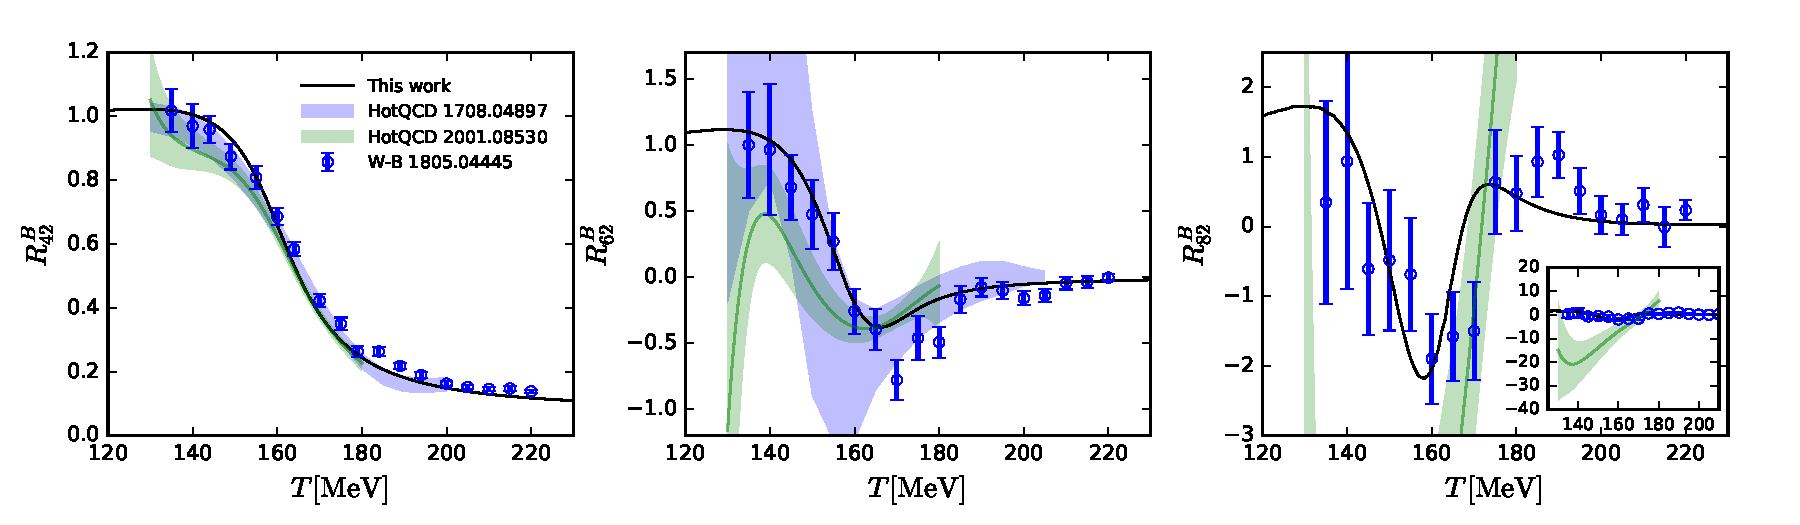
\includegraphics[width=1\textwidth]{R42R62R82-T-muB0}
\caption{$R^{B}_{42}=\chi^{B}_{4}/\chi^{B}_{2}$ (left panel), $R^{B}_{62}=\chi^{B}_{6}/\chi^{B}_{2}$ (middle panel), and $R^{B}_{82}=\chi^{B}_{8}/\chi^{B}_{2}$ (right panel) as functions of the temperature with vanishing baryon chemical potential ($\mu_B=0$). Results obtained with the low energy effective theory within fRG approach are compared with lattice results from the HotQCD collaboration \cite{Bazavov:2017dus,Bazavov:2017tot,Bazavov:2020bjn} and the Wuppertal-Budapest collaboration \cite{Borsanyi:2018grb}. The inset in the plot of $R^{B}_{82}$ shows its zoom-out view.}\label{fig:R42R62R82-T-muB0}
\end{figure*}
%%%%%%%%%%%%%%%%%%%%%%%%%%%%%
%


In this section we would like to present our calculated results and compare them with the relevant lattice calculations. Implications of our prediction for the hyper-order baryon number fluctuations in the heavy-ion collision experiments will also be discussed. But before we do that, the scales in the LEFT and OCD have to be matched.

\subsection{Matching the scales in LEFT and OCD}
\label{subsec:scale}

Usually the scale in LEFT and that in QCD do not agree with each other exactly, and a direct consequence is that the pseudocritical temperature of the chiral phase crossover, i.e., the value of $T_c$ at $\mu_B=0$ is different in the LEFT and QCD. Although it is not a real phase transition, the benchmark value of $T_c$ is well determined through, e.g., the chiral condensate, chiral susceptibilities, etc. Recently, two lattice collaborations, the HotQCD collaboration and the Wuppertal-Budapest collaboration find $T_c=156.5\pm 1.5$ MeV \cite{Bazavov:2018mes} and $T_c=158.0\pm 0.6$ MeV, respectively. Furthermore, the scale is also affected by the number of quark flavors. As shown in the effective action in \Eq{eq:action}, only the $N_f=2$ flavor quarks, i.e., light quarks $u$ and $d$, are included in the LEFT in this work, while in lattice simulations besides the light quarks, dynamics of the strange quark is also taken into account. Thus there should be a mismatch of the scale resulting from the different systems of $N_f=2$ and $N_f=2+1$ flavor quarks.

We denote the temperature and the baryon chemical potential in the LEFT as $T_{_{LEFT}}$ and $\mu_{B_{LEFT}}$, respectively, where the suffix is used to distinguish them from $T$ and $\mu_{B}$ in QCD or lattice simulations. In order to resolve the mismatch of the scale in LEFT and OCD, a simple linear relation between them both for the temperature and chemical potential is assumed, to wit,
%
\begin{align}
  T_{_{LEFT}}&=c_{_{T}}T\,, \quad \mu_{B_{LEFT}}=c_{\mu}\mu_{B}\,,\label{eq:rescale}
\end{align}
%
where the constant coefficients $c_{_{T}}$ and $c_{\mu}$ are to be determined.

The coefficient $c_{_{T}}$ in \Eq{eq:rescale} is fixed through fitting the LEFT curve of $R^{B}_{42}=\chi^{B}_{4}/\chi^{B}_{2}$ in the left panel of \Fig{fig:R42R62R82-T-muB0}, i.e., the kurtosis of the baryon number distribution $\kappa \sigma^2=R^{B}_{42}$, 
as a function of the physical temperature $T$ with $\mu_B=0$ in comparison to the lattice results. It is found that the LEFT within fRG provides the best description of the lattice $\kappa \sigma^2$ with $c_{_{T}}=1.247(12)$. To proceed, the constant $c_{\mu}$ in \Eq{eq:rescale} is determined by the curvature of the phase boundary, which is defined as the quadratic expansion coefficient of the pseudocritical temperature as a function of the baryon chemical potential around $\mu_B=0$, i.e.,
%
\begin{align}
  \frac{T_c(\mu_B)}{T_c}&=1-\kappa \left(\frac{\mu_B}{T_c}\right)^2+\lambda \left(\frac{\mu_B}{T_c}\right)^4+\cdots\,,\label{eq:curv}
\end{align}
%
with the curvature $\kappa$, where the next fourth order expansion coefficient $\lambda$ is neglected in our calculations, since it hardly plays any role in the region of baryon chemical potential concerned in this work, e.g., up to $\mu_B\sim 400$ MeV in the following, due to its small value. $T_c$ in \Eq{eq:curv} is the pseudocritical temperature at $\mu_B=0$. Note that the curvature is invariant only if the chemical potential and temperature are rescaled with the same value, and thus the curvature $\kappa_{_{LEFT}}$ in the LEFT would not be modified if one has $c_{\mu}=c_{_{T}}$ in \Eq{eq:rescale}. By employing the renormalized light quark condensate, we obtain $\kappa_{_{LEFT}}=0.0193$ in the $N_f=2$ flavor LEFT. For more discussions about the renormalized light quark condensate and its related phase boundary, see, e.g., \cite{Fu:2019hdw}. This value of $\kappa_{_{LEFT}}$ is a bit larger than recent $N_f = 2+1$ lattice results, e.g., $\kappa=0.015(4)$ in \cite{Bazavov:2018mes}, $\kappa=0.0149(21)$ in \cite{Bellwied:2015rza}, $\kappa=0.0153(18)$ in \cite{Borsanyi:2020fev}. This mismatch of the curvature between the LEFT and lattice QCD, however, is cured through a suitable choice for the ratio $c_{\mu}/c_{_{T}}$ in \Eq{eq:rescale}, and one readily arrives at
%
\begin{align}
  c_{\mu}&=c_{_{T}}\left(\frac{\kappa}{\kappa_{_{LEFT}}}\right)^{1/2}\,.\label{eq:cmu}
\end{align}
%
Substituting $\kappa_{_{LEFT}}=0.0193$, $\kappa=0.0153(18)$, and $c_{_{T}}=1.247(12)$ into the equation above, one obtains $c_{\mu}=1.110(66)$.

To sum up, in this section the scales between the LEFT and QCD have been matched by resorting to two observables, i.e., $R^{B}_{42}$ as a function of $T$ at vanishing chemical potential and the curvature of phase boundary $\kappa$, which are both quite relevant to predictions of the hyper-order baryon number fluctuations at finite temperature and densities, to be discussed in the following. 

%%%%%%%%%%%%%%%%%%%%%%%%%%%%%%%%%%%%%%%%%%%%%%%%%%%%%%%%%%%%%
\subsection{Hyper-order baryon number fluctuations}
\label{subsec:hyper-order}

%
%%%%%%%%%%%%%%%%%%%%%%%%%%%%%
\begin{figure*}[t]
\centering
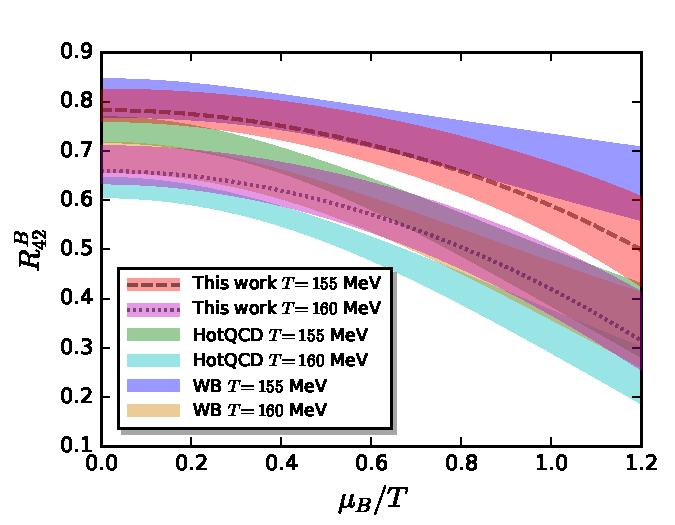
\includegraphics[width=0.85\columnwidth]{R42-muBoT} 
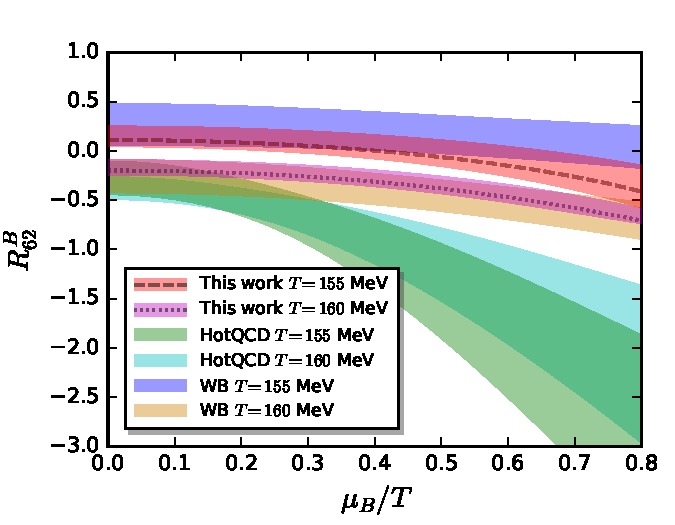
\includegraphics[width=0.85\columnwidth]{R62-muBoT} 
\caption{$R^{B}_{42}$ (left panel) and $R^{B}_{62}$ (right panel) as functions of $\mu_B/T$ with $T=155$ MeV and $T=160$ MeV. Calculation of LEFT within the fRG approach is compared with lattice QCD computations by the HotQCD collaboration \cite{Bazavov:2020bjn} and the Wuppertal-Budapest collaboration \cite{Borsanyi:2018grb}.
} \label{fig:R42R62-muBoT}
\end{figure*}
%%%%%%%%%%%%%%%%%%%%%%%%%%%%%
%

%
%%%%%%%%%%%%%%%%%%%%%%%%%%%%%
\begin{figure*}[t]
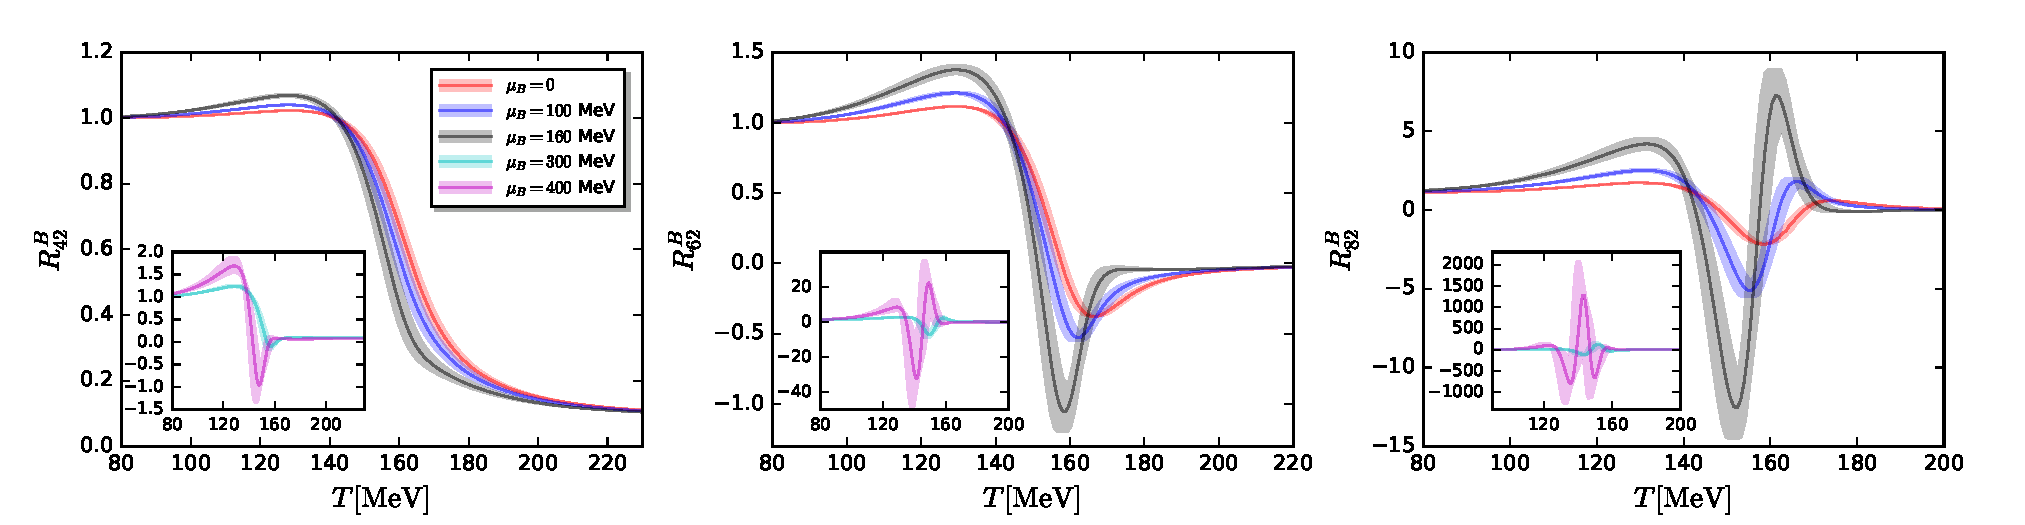
\includegraphics[width=1.\textwidth]{R42R62R82-T-muB}
\caption{$R^{B}_{42}$ (left panel), $R^{B}_{62}$ (middle panel), and $R^{B}_{82}$ (right panel) as functions of the temperature at several values of $\mu_B$, computed from LEFT within the fRG approach.}\label{fig:R42R62R82-T-muB}
\end{figure*}
%%%%%%%%%%%%%%%%%%%%%%%%%%%%%
%



As we have discussed above, the LEFT has been calibrated by use of the curvature of phase boundary and the kurtosis of baryon number distribution as a function of $T$ with $\mu_B=0$, via a detailed comparison with recent lattice results. Consequently, one could use the LEFT to make predictions for the dependence of $R^{B}_{42}$ on the chemical potential, as well as the hyper-order baryon number fluctuations at finite temperature and density. In the middle and right panels of \Fig{fig:R42R62R82-T-muB0}, $R^{B}_{62}=\chi^{B}_{6}/\chi^{B}_{2}$ and $R^{B}_{82}=\chi^{B}_{8}/\chi^{B}_{2}$ are shown versus the temperature with vanishing $\mu_B$, respectively, and in the same way the LEFT and lattice QCD results are compared. Apparently, one observes that, with the increase of the order of fluctuations, errors of lattice calculation increase dramatically. Especially, the eighth-order fluctuations $R^{B}_{82}$ obtained by the two collaborations show a significant quantitative difference, although they are roughly consistent with each other qualitatively. It is found that the predicted hyper-order baryon number fluctuations from the LEFT within the fRG, are in qualitative agreement with both lattice results, and even consistent with the Wuppertal-Budapest result quantitatively within the errors.

To proceed, we consider the chemical potential dependence of baryon number fluctuations. Expanding the pressure in \Eq{eq:pres} in powers of $\hat{\mu}_{B}\equiv\mu_B/T$ around $\hat{\mu}_{B}=0$ , one is led to 
%
\begin{align}
  \frac{p}{T^4}&=\frac{p}{T^4}\Big|_{\hat{\mu}_{B}=0}+\sum_{i=1}^{\infty}\frac{\chi^B_{2i}|_{\hat{\mu}_{B}=0}}{(2i)!}\hat{\mu}_{B}^{2i}\,.\label{eq:cmu}
\end{align}
%
Truncating the Taylor expansion above up to order of $\hat{\mu}_{B}^{8}$ and employing \Eq{eq:suscept}, we obtain the expanded baryon number fluctuations in the first several orders, to wit,
%
\begin{align}
\chi^B_2\simeq&\chi^B_2|_{\hat{\mu}_{B}=0}+\frac{\chi^B_4|_{\hat{\mu}_{B}=0}}{2!}\hat{\mu}_{B}^{2}+\frac{\chi^B_6|_{\hat{\mu}_{B}=0}}{4!}\hat{\mu}_{B}^{4}\nonumber\\[2ex]
&+\frac{\chi^B_8|_{\hat{\mu}_{B}=0}}{6!}\hat{\mu}_{B}^{6}\,,\label{}\\[2ex]
\chi^B_4\simeq&\chi^B_4|_{\hat{\mu}_{B}=0}+\frac{\chi^B_6|_{\hat{\mu}_{B}=0}}{2!}\hat{\mu}_{B}^{2}+\frac{\chi^B_8|_{\hat{\mu}_{B}=0}}{4!}\hat{\mu}_{B}^{4}\,,\\[2ex]
\chi^B_6\simeq&\chi^B_6|_{\hat{\mu}_{B}=0}+\frac{\chi^B_8|_{\hat{\mu}_{B}=0}}{2!}\hat{\mu}_{B}^{2}\,.\label{}
\end{align}
%
In \Fig{fig:R42R62-muBoT} we show the lattice results $\chi^B_4/\chi^B_2$ and $\chi^B_6/\chi^B_2$ based on the Taylor expansion above, and the fluctuations at vanishing chemical potential, viz. $\chi^B_{i}|_{\hat{\mu}_{B}=0}$ ($i=2$, 4, 6, 8) and relevant results in \Fig{fig:R42R62R82-T-muB0}, from the HotQCD collaboration \cite{Bazavov:2020bjn} and the Wuppertal-Budapest collaboration \cite{Borsanyi:2018grb}. Moreover, $\chi^B_n$'s in \Eq{eq:suscept} could also be computed directly in the LEFT within the fRG approach, without resorting to the Taylor expansion, and the relevant results are presented in \Fig{fig:R42R62-muBoT} for comparison. Here we choose two values of the temperature, and as expected, the LEFT result for the dependence of $R^{B}_{42}$ and $R^{B}_{62}$ on the chemical potential, agrees with both lattice results qualitatively, and is even quantitatively consistent with the Wuppertal-Budapest result.

In \Fig{fig:R42R62R82-T-muB} $R^{B}_{42}$, $R^{B}_{62}$ and $R^{B}_{82}$ are depicted as functions of $T$ with several values of $\mu_B$, which are calculated in LEFT with the fRG approach. Relevant results in \Fig{fig:R42R62R82-T-muB0} for $\mu_B=0$ are presented as well, in order to highlight effects of the finite baryon chemical potential. One observes that both the magnitude and error of the fluctuations, in particular the high-order ones, grow larger with the increasing chemical potential.





 





%The coefficient $c_{_{T}}$ in \Eq{eq:rescale} is fixed through the relative values of the pseudocritical temperature at $\mu_B=0$ in the LEFT and QCD, i.e., $c_{_{T}}=T_{c_{LEFT}}/T_c$, where $T_c=156$ MeV is employed for QCD from the lattice simulations. Hence, determination of $T_{c_{LEFT}}$ in the LEFT plays a key role in fixing the coefficient $c_{_{T}}$. Unfortunately, the chiral phase transition with the temperature at $\mu_B=0$ is not an exact phase transition, but rather a continuous crossover, due to a finite current quark mass. Accordingly, different observables might result in nonidentical $T_{c_{LEFT}}$. Since we are concerned with the baryon number fluctuations in this work, the kurtosis of the baryon number distribution, i.e., $\kappa \sigma^2=\chi_4^{B}/\chi_2^{B}$, is used to fix $T_{c_{LEFT}}$ as follows. In the left panel of \Fig{fig:R42R62R82-T-muB0}, $\chi_4^{B}/\chi_2^{B}$ is shown as a function of the temperature in unit of $T_c$ with vanishing baryon chemical potential, and result of the LEFT within fRG is compared with that of lattice QCD. It is found that the LEFT within fRG gives the best description of $\kappa \sigma^2$ in comparison to the lattice results with $T_{c_{LEFT}}=195$ MeV, which yields  
%\begin{align}
%  c_{_{T}}&=T_{c_{LEFT}}/T_c=1.25\,.\label{eq:cT}
%\end{align}
%From now on unless explicitly specified, values of temperature in the following, e.g., in legends of figures, are always referred to $T$, and the relevant $T_{_{LEFT}}$ in the LEFT could be inferred from Eqs. (\ref{eq:rescale}) and (\ref{eq:cT}).

 





























%
 %%%%%%%%%%%%%%%%%%%%%%%%%%%%
%\begin{figure*}[t]
%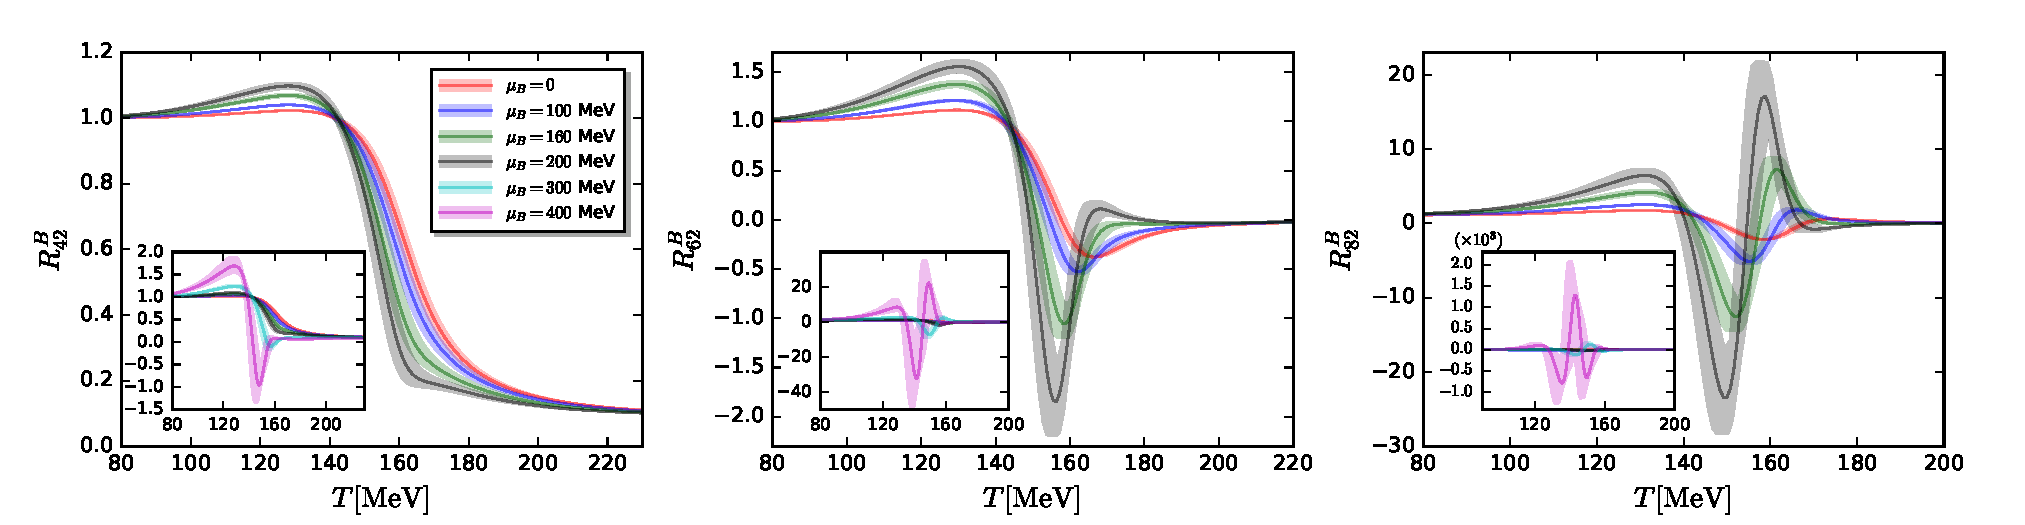
\includegraphics[width=1\textwidth]{R42R62R82-T-muB0to400}
%\caption{Evolution of the dependence of $\chi^{B}_{4}/\chi^{B}_{2}$ (left panel), $\chi^{B}_{6}/\chi^{B}_{2}$ (middle panel), and $\chi^{B}_{8}/\chi^{B}_{2}$ (right panel) on the temperature, with the increasing $\mu_B$ from 0 to 400 MeV.}\label{fig:R42R62R82-T-muB0to400}
%\end{figure*}
%%%%%%%%%%%%%%%%%%%%%%%%%%%%%
%

%
 %%%%%%%%%%%%%%%%%%%%%%%%%%%%
%\begin{figure*}[t]
%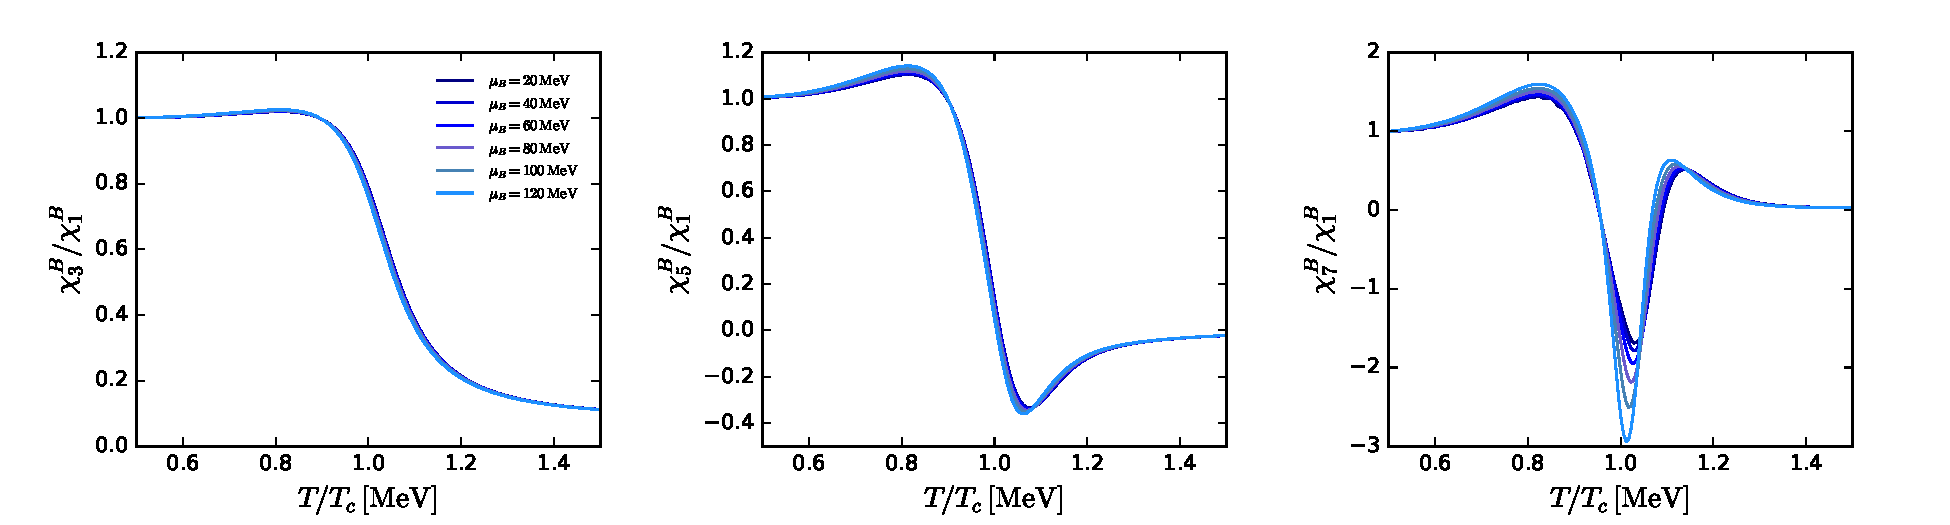
\includegraphics[width=1\textwidth]{R31R51R71-T-muB0to120}
%\caption{$\chi^{B}_{3}/\chi^{B}_{1}$ (left panel), $\chi^{B}_{5}/\chi^{B}_{1}$ (middle panel), and $\chi^{B}_{7}/\chi^{B}_{1}$ (right panel) as functions of the temperature with some selective values of $\mu_B$ from 0 to 120 MeV.}\label{fig:R31R51R71-T-muB0to120}
%\end{figure*}
%%%%%%%%%%%%%%%%%%%%%%%%%%%%%
%

%
 %%%%%%%%%%%%%%%%%%%%%%%%%%%%
%\begin{figure*}[t]
%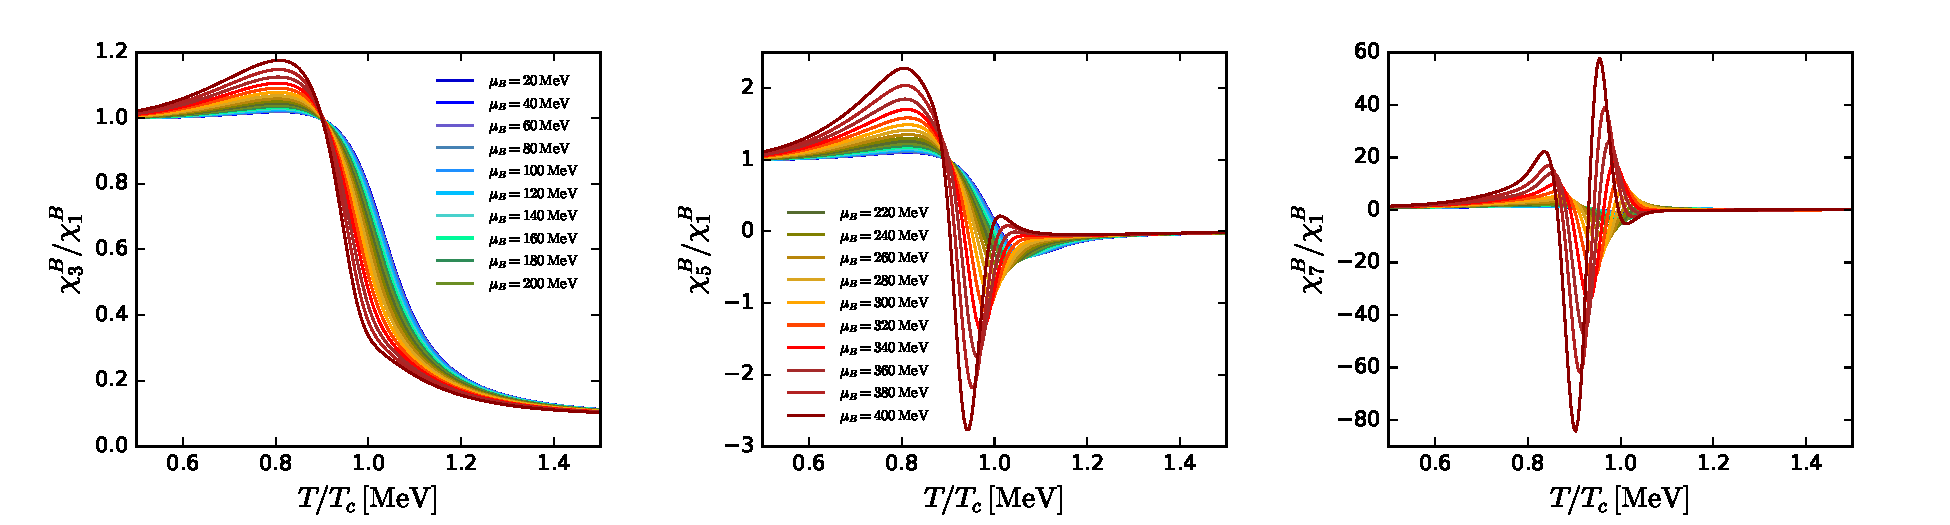
\includegraphics[width=1\textwidth]{R31R51R71-T-muB0to400}
%\caption{Evolution of the dependence of $\chi^{B}_{3}/\chi^{B}_{1}$ (left panel), $\chi^{B}_{5}/\chi^{B}_{1}$ (middle panel), and $\chi^{B}_{7}/\chi^{B}_{1}$ (right panel) on the temperature, with the increasing $\mu_B$ from 20 to 400 MeV.}\label{fig:R31R51R71-T-muB0to400}
%\end{figure*}
%%%%%%%%%%%%%%%%%%%%%%%%%%%%%
%







%The results we show in \Fig{fig:mub0} is the kurtosis, i.e., the ratio of $\chi^B_4$ to $\chi^B_2$, then the ratio of $\chi^B_6$, $\chi^B_8$ to $\chi^B_2$ are given on the right. We use the kurtosis as a benchmark to fix our reduced temperature $T^{glue}_c$ and $\alpha$ in the gluon potential and the rescale $T_c$ of \Fig{fig:mub0}. On the basis of a well tally of the kurtosis, the $\chi^B_6/\chi^B_2$ and $\chi^B_8/\chi^B_2$ are compared. We introduce a rescale temperature $T_c=194$ MeV to remove the temperature difference between the lattice and the low energy effective model. We choose the $T_c$ by fitting the kurtosis with the lattice results. We find that the value of $T_c$ is related to the difference between the chiral phase transition temperature and confinement-deconfinement phase transition temperature. With the rising of the $T_c^{glue}$ and $\alpha$ in the glue potential, the difference between chiral phase transition temperature and deconfinement phase transition temperature decreases at the same time the rescale $T_c$ is rising. From the left diagram in the \Fig{fig:mub0} we can clearly see, the FRG result is better match with the Wuppertal-Budapest Collaboration results, but a little higher than the HotQCD Collaboration results, especially around the $T/T_c=0.9$ and $T/T_c=1.2$. In another word, the FRG result has a slow change rate compared with HotQCD result.\par
%The middle picture of \Fig{fig:mub0} is the comparision of the $\chi^B_6/\chi^B_2$. The FRG result is better match with two lattice results at low and high temperature. However, the values of the FRG around $T/T_c=1.0$ are not small enough to fit the lattice $\chi^B_6/\chi^B_2$. The valley depth of the FRG curve is related with the change rate of the kurtosis, i.e. the slow change rate of the kurtosis causes the shallow valley in the 6th order.\par
%The last picture in \Fig{fig:mub0} is the 8th order baryon number fluctuation. Here we only have the Wuppertal-Budapest Collaboration results. We can easily see from the picture, FRG is match well with lattice, except around $T/T_c=1.2$, FRG curve is lower than the lattice. We believe the reason of the difference is also the slow change rate of the kurtosis.\par
%The three pictures in \Fig{fig:finmu} is the FRG results under finite baryon chemical potential from $0$ to $400$ MeV. As seen in left picture, the kurtosis grow high around $T/T_c=0.8$ and become lower around $T/T_c=0.95$. The behavior of the kurtosis under PQM model is also discussed in \cite{Fu:2015amv}. The change of the peak and valley values of the kurtosis lead to the slope change of kurtosis. So it is obvious that the 6th and 8th order fluctuations gradually increase to big values.

%%%%%%%%%%%%%%%%%%%%%%%%%%%%%%%%%%%%%%%%%%%%%%%%%%%%%%%%%%%
%%%%%%%%%%%%%%%%%%%%%%%%%%%%%%%%%%%%%%%%%%%%%%%%%%%%%%%%%%%

\section{summary and outlook}
\label{sec:SO}

%%%%%%%%%%%%%%%%%%%%%%%%%%%%%%%%%%%%%%%%%%%%%%%%%%%%%%%%%%%
%%%%%%%%%%%%%%%%%%%%%%%%%%%%%%%%%%%%%%%%%%%%%%%%%%%%%%%%%%%

\begin{acknowledgments}

The work was supported by the National Natural Science Foundation of China under Contracts Nos. 11775041.

\end{acknowledgments}

%%%%%%%%%%%%%%%%%%%%%%%%%%%%%%%%%%%%%%%%%%%%%%%%%%%%%%%%%%%%%
%%%%%%%%%%%%%%%%%%%%%%%%%%%%%%%%%%%%%%%%%%%%%%%%%%%%%%%%%%%%%

\appendix

\section{Glue potential}
\label{app:gluepot}


Now come to the gluon part, we involve the gluon effect by the glue potential which is related to the Polyakov loop with temporal gluonic background $A_0$
\begin{align}
L(\bm x)=\frac{1}{N_c}\langle \Tr{\mathcal{P}(\bm x)} \rangle ,\qquad \bar{L} (\bm x)=\frac{1}{N_c}\langle \Tr{\mathcal{P}^{\dagger}(\bm x)} \rangle\,,\label{}
\end{align}
the Polyakov loop has the form of
\begin{align}
\mathcal{P}(\bm x)=\mathcal{P}\exp\bigg( ig\int_{0}^{\beta}d\tau A_0(\bm x,\tau) \bigg)\,.\label{}
\end{align}
The glue potential which we employed in the model, see \cite{Lo:2013hla}, is parameterized as the form below
\begin{align}
U_{glue}(L,\bar{L})/T^4=&-\frac{a(T)}{2}\bar{L}L+b(T)\mathrm{ln}M_H(L,\bar{L})\nonumber \\ 
&+\frac{c(T)}{2}(L^3+\bar{L}^3)+d(T)(\bar{L}L)^2.
\end{align}
$M_H(L,\bar{L})$ stands for the Haar measure which is defined as
\begin{align}
M_H(L,\bar{L})=1-6\bar{L}L+4(L^3+\bar{L}^3)-3(\bar{L}L)^2.
\end{align}
Then we give the parametric form of the factors of the $a,b,c,d$. The factor $a,c,d$ have the same form
\begin{align}
x(T)=\frac{x_1+x_2/t_c+x_3/t_c^2}{1+x_4/t_c+x_5/t_c^2},
\end{align}
and the form of $b$ is
\begin{align}
b(T)=b_1 t_c^{-b_4}(1-e^{b_2/t_c^{b_3}}),
\end{align}
the values of the parameters are fixed by the thermodynamics and can be found at \cite{Lo:2013hla}. The temperature $t_c$ is reduced temperature by $t_c=(T-T_c)/T_c$. We rescale the reduced temperature to make the glue potential accord with the Yang-Mills theory by $(t_c)_{YM}\rightarrow \alpha(t_c)_{glue}$, and $(t_c)_{glue}=(T-T^{glue}_c)/T^{glue}_c$. Here we choose $\alpha=0.7$ and $T^{glue}_c=270\,\mathrm{MeV}$ by fitting the kurtosis of the baryon number fluctuation with the lattice results. The effect of the Polyakov loop is working on the fermion distribution function see \cite{Fu:2015naa}. 







%%%%%%%%%%%%%%%%%%%%%%%%%%%%%%%%%%%%
\section{Threshold functions}
\label{app:thresholdfun}

For the purpose of solving the flow equation of the effective potential \Eq{eq:flowV} we use the Tylor expansion approach around the expansion point $\kappa$. The renormalised effective potential under the Tylor expansion is
\begin{align}
\bar{U}_k(\bar{\rho})=\sum^{N_u}_{n=0}\frac{\bar{\lambda}_{n,k}}{n!}(\bar{\rho}-\bar{\kappa}_k)^n,\label{eq:Tylor}
\end{align}
with $\bar{U}_k(\bar{\rho})=U_k(\rho)$, $\bar{\lambda}_{n,k}=\lambda_{n,k}/(Z_{\phi,k})^n$, $\bar{\rho}=Z_{\phi,k}\rho$, $\bar{\kappa}_k=Z_{\phi,k}\kappa_k$.
Here we take $N_u=5$ for the well convergence of effective potential. The running cutoff scale dependent expansion point $\kappa_k$ is emploied in our numerical calculation. Then we can get the Tylor expansion flow equation from \Eq{eq:flowV} and \Eq{eq:Tylor} 
\begin{align}
&\partial^n_{\bar{\rho}}\bigg(\partial_t |_\rho\bar{U}_k(\bar{\rho})\bigg)\bigg|_{\bar{\rho}=\bar{\kappa}_k}\nonumber\\[2ex]
=&(\partial_t-n\eta_{\phi,k})\bar{\lambda}_{n,k}-(\partial_t\bar{\kappa}_k+\eta_{\phi,k}\bar{\kappa}_k)\bar{\lambda}_{n+1,k}\,.\label{eq:drhodu}
\end{align}
There is another chosen of the expansion point i.e. fixed point which the bare $\kappa$ is independent on the cutoff scale which has a good convergence property of $N_u$, see, e.g.\cite{Pawlowski:2014zaa,Yin:2019ebz}. However, the fixed point expansion may introduce temperature dependence into the Tylor expansion and the thermodynamics will be influence by this property, so we choose the running point expansion in this work. The running point is the solution of the equation of motion
\begin{align}
\frac{\partial}{\partial \bar{\rho}}\bigg( \bar{U}_k(\bar{\rho})-\bar{c}_k(2\bar{\rho})^{\frac{1}{2}}\bigg)\bigg|_{\bar{\rho}=\bar{\kappa}_k}=0\,.\label{eq:EoM}
\end{align}
We emphasize that the equation of motion must be satisfied under every value of the infrared cutoff. The renormalised explicit symmetry breaking term is $\bar{c}_k=c/(Z_{\phi,k})^{1/2}$, with the flow $\partial_t \bar{c}_k=(1/2)\eta_{\phi,k}\bar{c}_k$. From \Eq{eq:drhodu} and \Eq{eq:EoM} we can obtain the flow of the renormalised running expansion point
\begin{align}
  \partial_t \bar \kappa_k&=-\frac{\bar c_k^2}{\bar{\lambda}_{1,k}^3+\bar c_k^2\bar{\lambda}_{2,k}}\bigg[\partial_{\bar \rho}\left(\partial_t\big|_{\rho} \bar U_k(\bar \rho)\right)\bigg|_{\bar \rho=\bar \kappa_k}\nonumber \\[2ex]
  &+\eta_{\phi,k}\left(\frac{\bar{\lambda}_{1,k}}{2}+\bar\kappa_k\bar{\lambda}_{2,k}\right)\bigg]\,.\label{}
\end{align}
In this work we don't consider the field dependence of the Yukawa coupling and the renormalised Yukawa coupling is $\bar{h}_k=h_k/(Z_{\psi,k}Z^{1/2}_{\phi,k})$.\par
Now we give the ultraviolet of the flow equations i.e. the initial conditions of the differential equations. The ultraviolet cutoff scale is set to $\Lambda=700\,\mathrm{MeV}$. The parameterized effective potential at UV point is
\begin{align}
U_{k=\Lambda}(\rho)=\frac{\lambda_{k=\Lambda}}{2}\rho^2+\nu_{k=\Lambda}\rho\,,
\end{align}
The values of the parameters in the effective potential are $\lambda_{k=\Lambda}=11$ and $\nu_{k=\Lambda}=(0.830\,\mathrm{GeV})^2$. In addition, the initial values of the explicit chiral symmetry breaking strength and Yukawa coupling are $c=2.82\times 10^{-3}\,\mathrm{GeV}^3$ and $h_{k=\Lambda}=10.18$. These parameters are fixed by fitting the vacuum physical observables, i.e., $f_\pi=92\,\mathrm{MeV}$, $m_\psi=300\,\mathrm{MeV}$, $m_\pi=136\,\mathrm{MeV}$,and $m_\sigma=479\,\mathrm{MeV}$.



%%%%%%%%%%%%%%%%%%%%%%%%%%%%%%%%%%%%%%%%%%%%%%%%%%%%%%%%%%%%%%%%
%%%%%%%%%%%%%%%%%%%%%%%%%%%%%%%%%%%%%%%%%%%%%%%%%%%%%%%%%%%%%%%%
% The \nocite command causes all entries in a bibliography to be
% printed out whether or not they are actually referenced in the
% text. This is appropriate for the sample file to show the different
% styles of references, but authors most likely will not want to use
% it.  \nocite{*}

%\bibliography{refspec}% Produces the bibliography via BibTeX.
\bibliography{ref-lib}% Produces the bibliography via BibTeX.


\end{document}
